\documentclass{article}

\usepackage{epsfig} \usepackage[margin=1.5in]{geometry}
\usepackage[round]{natbib}
\usepackage{amsmath}
\usepackage{amsfonts}
\usepackage{cleveref}
\usepackage{verbatim}
\usepackage{float}

\newcommand{\bO}{\mathcal{O}}
\newcommand{\argmin}[1]{\underset{#1}{\operatorname{arg\;min}}\;}

\title{Computational Methods for Principle Component Analysis Applied to
  Genotype Data}
\date{}

\begin{document}

\maketitle

\section{Introduction}

Population stratification (PS) is an important confounder for the association  between
genotypes and phenotypes \citep{price2006principal}.
To adjust for PS, we need to accurately estimate the ancestry structure in the study samples. Principle component analysis (PCA) is a multivariate statistical method which finds the direction of the maximum variability. By aggregating information across all genetic markers, PCA can accurate infer the ancestry structure \citep{reich2008principal}.
To adjust for PS, PCA can be applied to study data to calculate PC scores, which are regarded as variables of ancestry direction and can be used as covariates to adjust for. An alternative approach is predicting the PC scores of the study samples using reference genotyped samples with detailed ancestry information.
This prediction-based approach not only allows to adjust for PS but also to infer ancestry memberships of study samples. 

The standard way of predicting PC scores is to find the PC loadings of the reference data and project the data points of the study samples onto them.
We call this method simple projection (SP).
However, when the number of features are greatly larger than the size of the reference sample,
the predicted PC scores by this method are known to be biased toward null \citep{dey2016asymptotic}.
One way of addressing this shrinkage bias is presented by \citet{wang2014ancestry, wang2015improved}.
Their solution is to combine one study individual with the reference set and
find the PC scores of this augmented data set by singular value decomposition (SVD).
The PC scores of the study individuals are then retrieved from the singular vector matrices and mapped to the reference PC space by a Procrustes transformation.
We call this method ``augment, decompose, and Procrustes transform'' (ADP).
This method has been shown to be effective in eliminating the shrinking bias of
study PC scores.
However since ADP needs to run SVD for each study samples, ADP is computationally expensive.

To address the limitations of SP and ADP,
we propose and evaluate two alternative PC score prediction methods.
The first approach removes the bias in SP by estimating the asymptotic bias factor,
which is calculated based on Random Matrix Theory \citep{dey2016asymptotic}.
The second approach improves the computation efficiency of ADP by using online SVD algorithm \citep{halko2011finding}. 
We call the first approach ``adjusted projection'' (AP), and the second approach ``online augment, decompose, and Procrustes transform'' (OADP). 

In addition, we also address a computation problem with finding the PCs of the reference set when the reference sample sizes are large. 
The previously mentioned four methods all need to find the SVD of the reference data first.
This requires loading the covariance matrix of the reference data into the
computer's memory. 
However, when the size of the reference set is large,
the resulted covariance matrix will far exceed the size of a normal personal
computer's memory.
To solve this issue, a randomized SVD method has been developed that does not
require finding the covariance matrix.

In this paper, we compare the properties of
SP, ADP, AP, and OADP in terms of computation time and accuracy.
We also compare using standard SVD and randomized SVD for the reference set
and examine the difference in accuracy and computation time.
We found that AP and OADP have both achieved the accuracy of ADP
and the computational efficiency of SP.
In addition, randomized SVD gives results similar to standard SVD and only increase the computational time for the reference data.




\section{Method}

\subsection{Model}

\subsubsection{Data Format}
There are two genotype datasets, reference and study datasets, and both can be represented by matrices.
Suppose $X$ is a $p \times n$ matrix of reference genotypes and 
$Y$ is a $p \times m$ matrix of study sample genotypes, where 
$p$ is the number of genetic markers, $n$ is the number of reference samples and $m$ is the number of study samples. Each entry of $X$ and $Y$ is the number of minor alleles (0,1,2) of single nucleotide polymorphism (SNP). 
For genotype data, it is common for $p$ to be significantly larger than either $n$ or $m$.
Thus we assume this to be true except for the part where we discuss the randomized SVD algorithm,
which is developed to handle datasets with exceedingly large $n$.

\subsubsection{Principle Component Analysis}\label{pca-intro}
Given a multi-dimensional data, PCA searches for the directions in which the data has the greatest variance.
These unit vectors are called the principle components (PCs).
The PC's form an orthonormal basis for the sample space,
and we can ignore all but the first few PC's to reduce the dimension of the data.
In particular, let $X$ be standardized so that each row (feature) has mean equal to zero and standard deviation equal to one.
Moreover, Let $X=UDV^T$ be the SVD of $X$,
where $U$ is a $p \times n$ matrix whose columns are the PC's,
$D$ is an $n \times n$ diagonal matrix storing the standard deviations of the PC's,
and $V$ an $n \times n$ matrix such that each row contains the standardized PC scores of an individual.
(Alternatively, we can use eigendecomposition to find the matrices since $X^T X = VD^2V^T$ and $X X^T = UD^2U^T$.)
We sort the diagonal elements of $D$ in descending order and rearrange the
columns of $U$ and $V$ accordingly.
We are interested in the top $k$ PC's (where $k \ll n$) and look at the top $k$
columns of $V$ for their PC scores.

\subsubsection{Estimating PC scores}

population.
In the ideal case in which the genotypes of all individuals of the population are given
we use the method in \Cref{pca-intro} to find the PC scores of the individuals
we are interested in.
In practice, however, we have a reference dataset and a study dataset assumed to be generated from the
same population and use the former to estimate the populational PC scores of the latter.
There are several computational methods one can use to do this estimation.
In \Cref{sec:compu}, we compare the performance of four of them.

\subsection{Computational Methods}\label{sec:compu}



\subsubsection{Simple Projection (SP)}
The standard way for estimating PC scores is by projecting the study
individuals' data points to the PC space of the reference individuals by using reference sample PC loadings,
which is the matrix $U$ in the eigendecomposition of the (standardized) reference sample matrix $X$.
The PC loadings are unit vectors pointing toward the directions of the greatest variances in the $p$-dimension sample space.
We call this method ``simple projection'' (SP).
The algorithm goes as follows.

\begin{enumerate}
\item Compute $X^T X$.
  (Computational complexity: $\bO[n^2p]$.)  
\item Apply eigendecomposition to $X^T X$ to get $X^T X = V D^2 V^T$.
  ($\bO[n^3]$.)
\item Calculate PC loading matrix $L = X V_1 D_1^{-1}$,
where $V_1$ and $D_1$ are the the first $k_1$ columns of $V$ and $D$, respectively ($\bO[k_1^2 n + knp]$)
\item Calculate predicted PC scores $W = Y^T L$, where $Y$ is the data matrix for all the study individuals ($\bO[mpk_1]$.)
\end{enumerate}

Total computational complexity: 
\[
    \bO[n^2p + n^3 + k_1^2 n + pnk_1 + pmk_1)] \approx \bO[n^2p + mk_1p]
\]
given that $k_1 \ll n \ll p$.

As the reference sample size increases,
the computational complexity of SP stays as a constant,
except for decomposing the reference matrix, which is done once for all study individuals.
However, it is known that the projection method tends to underestimates the magnitude of the PC scores when $n \ll p$ \citep{dey2016asymptotic},
which we call the ``shrinking bias''.
This limits the accuracy of SP for high dimensional data.

\subsubsection{Augment, Decompose, and Transform (ADP)}

One way to solve the shrinking bias of SP is the ADP approach developed by \citet{wang2014ancestry, wang2015improved}.
In this method, each study individual's data point is appended to the reference
data matrix.
Then SVD is applied to the augmented matrix,
and PC scores in this augmented sample are found for both the reference
individuals and the study individual.
The the PC scores of the reference individuals in this augmented sample is
compared with the PC scores of the reference individuals in the reference
sample,
which is calculated in the beginning,
and a linear (Procrustes) map is constructed to transform the latter into the former
with the smallest error.
This transformation is then applied to the PC scores of the study individual in
the augmented sample.
The resulted PC scores are used as an estimate for the study individual's
population PC scores.
Specifically, let
\[
  V =
  \begin{bmatrix}
    V_{\text{ref}} & W
  \end{bmatrix},
  \quad
  \tilde{V} =
  \begin{bmatrix}
    \tilde{V}_{\text{ref}} & \tilde{W}_\text{ref} \\
    \tilde{V}_\text{stu} & \tilde{W}_\text{stu}
  \end{bmatrix},
\]
where the dimensions of $V_\text{ref}$, $\tilde{V}_\text{ref}$, and $\tilde{V}_\text{stu}$ are $n \times k_1$, $n \times k_2$, and $1 \times k_2$, respectively, with $ 1 \leq k_1 \leq k_2 \leq n+1$. 
Next, we use Procrustes analysis to find
\[
  A, b = \argmin{A, b} d(V_\text{ref}, \tilde{V}_{\text{ref}}A+b)
\]
for some metric $d$.
Finally, we get the Procrustes-adjusted top $k_1$ PC scores for the study individual $V_\text{pro} = \tilde{V}_\text{stu} A + b$.
The algorithm is summarized as follows:
\begin{enumerate}
\item Compute $X^T X$.
  (Computational complexity: $\bO[n^2p]$.)  
\item Apply eigendecomposition to $X^T X$ to get $X^T X = V D^2 V^T$ (columns of $D$ and $V$ are sorted by PC variance with the first column corresponding to the greatest PC variance).
  ($\bO[n^3]$.)
\item Append $X^T y$ and its transpose to the last column and row of $X^T X$, respectively.
  The entry of the bottom-right corner is $y^T y$.
  This is exactly the same as computing $\tilde{X}^T \tilde{X}$,
  where $\tilde{X} = (X, y)$ is the reference group with the study individual added.
  ($\bO[np]$.)
\item Apply eigendecomposition to $\tilde{X}^T \tilde{X}$ to get $\tilde{X}^T \tilde{X} = \tilde{V} \tilde{D}^2 \tilde{V}^T$.
  ($\bO[n^3]$.)
\item Project the first $k_2$ columns of $\tilde{V}$ to the first $k_1$ columns of $V$ by using Procrustes analysis to get the transformed PC scores of the study individual (the last row of $V$),
  where $k_1 < k_2 \ll n$.
  (Computational complexity is ignorable if $k_2$ is not large compared to $n$.)
  \item Go to step 3 for the next study individual.
\end{enumerate}

Total Computational complexity: $\bO[n^2p + m(np + n^3)]$.

Although accurate, ADP is the slowest among the other three computational methods.
Its computational complexity increases cubically with respect to the reference sample size and linearly with respect to the study sample size.
The ADP method is has been implemented in the TRACE software \citep{wang2014ancestry, wang2015improved}.


\subsubsection{Adjusted Projection (AP)}

A more efficient way to solve the shrinking bias of SP is to estimate the
magnitude and angle of the shrinkage and adjust the study individuals' PC scores accordingly.
This method has been developed by \citet{dey2016asymptotic} and implemented in the High
Dimension Principal Component Analysis (HDPCA) in the R language \citep{hdpca}.
HDPCA reads the PC scores and variances calculated by projection and estimate the shrinkage factor to restore the unshrinked scores. 
The algorithm is
\begin{enumerate}
\item Compute $X^T X$.
  (Computational complexity: $\bO[n^2p]$.)  
\item Apply eigendecomposition to $X^T X$ to get $X^T X = V D^2 V^T$.
  ($\bO[n^3]$.)
\item Calculate $W = Y^T (X V D_1^{-1})$, where $Y$ is the data matrix for all the study individuals, $D_1$ the first $k_1$ columns of $D$. ($\bO[mpk_1 + pnk_1]$.)
  \item Input $D$ and $W$ to the pc\_adjust function in the HDPCA function to obtain the PC scores adjusted for the shrinking bias. ($\bO[p]$ for finding the number of distant spikes (function select.nspike), $\bO[n]$ for adjusting for the shrinking bias (function hdpc\_est))
\end{enumerate}

Total computational complexity: $\bO[n^2p + mk_1(p + n) + p + n] \approx \bO[n^2p + mk_1p]$,
given that $m$ or $n$ is large. The computational complexities between simple projection and adjusted projection are the same.
The accuracy of adjusted projection will be empirically shown later.

\subsubsection{Online ADP (OADP)}

A remedy for ADP is to reduce the computational complexity without much sacrifice of the accuracy.
This is achieved by the online ADP (OADP) method.
Notice that in OADP, only the top $k_2$ PC's are used.
OADP uses the online SVD method, which calculates a close approximation of the first $k_3$ columns of $\tilde{V}$ for some $k_2 \leq k_3 \ll n$ and keeps everything else the same as in ADP, including Procrustes analysis. 
The algorithm is
\begin{enumerate}
\item Compute $X^T X$.
  (Computational complexity: $\bO[n^2p]$.)  
\item Apply eigendecomposition to $X^T X$ to get $X^T X = V D^2 V^T$.
  ($\bO[n^3]$.)
\item Calculate $U_3 = X V_3 D_3^{-1}$,
  where $V_3$ is the first $k_3$ columns of $V$,
  and $D_3$ is the diagonal matrix of the first $k_3$ diagonal entries of $D$.
  ($\bO[k_3 n p]$.)
\item Calculate 
  \[
    L = U_3^T y \quad \text{and} \quad K = y^T H,
  \]
  where $H$ is the normalized  $y - U_3L$
  ($\bO[k_3 p]$.)
\item Calculate $Q^T Q$, where
  \[
    Q = 
    \begin{bmatrix}
      D_3 & L \\
      0 & K
    \end{bmatrix}.
  \]
  ($\bO[k_3^3]$.)
\item Apply eigendecomosition to $Q^T Q$ to get $Q^T Q = \ddot{V}_3 \ddot{D}^2_3 \ddot{V}^T_3$.
  ($\bO[k_3^3]$.)
\item Calculate
  \[
    \tilde{V}_3 =
    \begin{bmatrix}
      V_3 & 0 \\
      0 & 1
    \end{bmatrix}
    \ddot{V}_3.
  \]
  ($\bO[nk_3^2]$.)
\item Project the first $k_2$ columns of $\tilde{V}_3$ to the first $k_1$ columns of $V$ by using Procrustes analysis to get the transformed PC scores of the study individual,
  where $k_1 < k_2  < k_3 \ll n$.
  (Computational complexity is ignorable if $k_2$ is not large compared to $n$.)
  \item Go to step 4 for the next study individual.
\end{enumerate}

Total computational complexity: $\bO[n^2p + n^3 + k_3np + m(k_3p + k_3^3 + nk_3^2]) \approx \bO[n^2p + m(k_3p + k_3^2n)]$, provided $k_3 \ll n \ll p$.

The computational complexity of OADP for the study individuals increases linearly with respect to the reference sample size, which makes the computation time of OADP close to those of SP.
The closeness between the results given by OADP and ADP will be empirically shown later.

A comparison of computational complexities of the four PCA methods are shown in \Cref{tbl:cplx}.

\subsubsection{Randomized SVD}

In addition to estimating the PC scores of the study individuals,
we have another algorithm that aims at improving the decomposition of the
training data.
For SP, AP, ADP, and OADP, we need to find the covariance matrix of the training
data, which has dimension $n \times n$, and conduct eigendecomosition on it.
However, when $n$ is exceedingly large,
computation and memory cost of PCA on the reference samples can be enormous.
A randomized SVD (RSVD) algorithm has been developed to handle this issue.
When the reference sample size is small, RSVD can be slower than standard SVD,
but it is scalable to large sample size.
For the details of the RSVD algorithm, see \citet{halko2011finding}.

Notice that the randomized SVD method on the training data
only calculates the first $k$ eigenvalues.
However, in order to use adjusted projection,
all the eigenvalues of the training data are required.
Thus for the missing eigenvalues,
we predict them by regressing their log-scale values on the ranks
and using the first $k$ eigenvalues for training the linear regression.


\section{Data}

In this study, we used both simulated data and real-life data to conduct
empirical tests of the computational methods for PCA.

\subsubsection{Simulation Studies}

We used the GGS software to simulate individuals migrating on a grid.
The parameters we chose to use are as follows:
\begin{enumerate}
\item L: Number of loci in each genealogy. (Fixed to $1000$.)
\item G: Number of genealogies. (Equal to $p / L$)
\item K: Side length of the grid. (Fixed to $2$.)
\item c: Number of haploids at each cell of the grid. (Equal to $2n / K^2$ and
$2m / K^2$)
\item M: Migration rate. (Fixed to $100$)
\end{enumerate}

For our study, we used different reference and study sample sizes.
First, we fix
the study size to be $m=200$ and increase $n$ from $1000$ to $3000$ with the
increment equal to $500$.
Next, we fix
the reference size to be $n=600$ and increase $m$ from $1000$ to $3000$ with the increment equal to $500$.

For comparing the speed of the algorithms,
we only compare the runtimes for the study individuals.
The time spent on calculations that are once-for-all (such as finding the SVD of
the reference matrix) is ignored.

For comparing the accuracy, we use two different measures.
First, for a given cell of the grid, we compute the mean of the PC scores of the 
reference individuals located at this cell.  
This is the estimated coordinate of the cell.
Next, we find the Euclidean distance between the estimated PC scores of the
study individuals and the estimated coordinates of the cells they are located
at.
These are the geographic estimation errors for the study individuals.
The average of these errors are used to measure the accuracy of the
computational methods (that is, the square root of the sum of squares divided by the
study size). 
Second, since ADP is a model free approach and believed to be the most reliable, we compare the average
Euclidean distance between the PC score estimates calculated by another method
to those calculated by ADP. 
The comparison of the runtimes and accuracy are also conducted by using both the
standard SVD and randomized SVD on the training data matrix.

\subsubsection{UK Biobank data analysis with 1000 Genomes as reference}

The real-life datasets used in our study are the UKBioBank and 1000 Genomes datasets.
They contain the genotype readings of individuals from different ethnic groups over the world.
For better comparison, we select only the SNPs that are included in both datasets,
the number of which is approximately $1.5 \times 10^5$.
We use the 1000 Genomes dataset as the reference and removed individuals who have at least one parent who is also in the dataset.
The reference samples size is approximately $2300$.
Moreover, we use the first 1000 individuals in the UKBioBank data set out of a
total number of $5 \times 10^5$ individuals. 
The measures we use for comparing speed and accuracy are the same as for
simulated data,
except that we do not use the geographic error here.
In addition, both the standard and randomized SVD on the training data set are tested.



\section{Results}

The predicted PC scores are shown in \Cref{fig:n1000} and \Cref{fig:ukb}.
For the comparison of the runtimes and accuracy for different reference and sample sizes for the simulated data,
see \Cref{fig:nChg} and \Cref{fig:mChg}.
For comparing the methods for the real-life data, see \Cref{tbl:ukb}.



\section{Discussion}

For the real-life datasets (\Cref{tbl:ukb} and \Cref{fig:ukb}),
we see that ADP, which is the most reliable method,
is the slowest in study runtimes.
By using the online SVD algorithm,
OADP achieved the highest accuracy (excluding ADP, which is the golden standard) and the fastest runtime.
SP is fast, also,
but its accuracy is the lowest.
By using the HDPCA package,
AP reduces the error of AP
and achieved the second highest in accuracy.
The randomized version of SP is as accurate as the standard SP,
which shows that the randomized SVD algorithm gives reliable results,
and that using linear regression to predict the uncalculated reference eigenvalues is satisfactory.
It also reduces the runtime almost by half,
due to not calculating all the eigenvalues.
Similar reduction in study runtime is observed for the randomized version of AP,
but in this case the accuracy is also decreased,
thought it is still higher than that of SP and RSP.
Finally, the randomized OADP is disappointing,
as its error is almost as high as SP and RSP.

The pattern for accuracy is very similar when we look at the simulated data.
(\Cref{tbl:nChg-runtimes-ref}, \Cref{tbl:nChg-runtimes-study},
\Cref{tbl:nChg-accuracy-gold}, \Cref{tbl:nChg-accuracy-ctr},
\Cref{tbl:mChg-runtimes-study}).
A noticeable difference in this case is the accuracy of ROADP.
Here ROADP's accuracy is almost identical to OADP's,
as measured by both the golden standard error and the geographic center err.
However, as the reference size increases,
the accuracies of different methods become closer and closer (\Cref{fig:nChg}).
As for the speed,
AWD's study runtime increases so fast with the reference size
that the study runtimes for the other methods seem to be constant in comparison (\Cref{fig:nChg}).
On the other hand,
the study runtimes appear to increase linearly with respect to the study size (\Cref{fig:mChg}).
This information can be used to predict the runtime for larger study samples.

\newpage

\bibliographystyle{plainnat}
\bibliography{frugalpca}


\newpage

\begin{table} 
  \centering
  \begin{tabular}{|l|l|l|}
    \hline
    Method & Reference Complexity & Study Complexity \\ 
    \hline
    ADP & $\bO[n^2 p]$ & $\bO[mn(p + n^2)]$ \\
    \hline
    OADP & $\bO[n^2 p]$ & $\bO[mk(p + k n)]$ \\
    \hline
    ROADP & $\bO[k^2 p]$ & $\bO[mk(p + k n)]$ \\
    \hline
    SP & $\bO[n^2p]$ & $\bO[mkp]$ \\
    \hline
    RSP & $\bO[k^2p]$ & $\bO[mkp]$ \\
    \hline
    AP & $\bO[n^2p]$ &  $\bO[mkp]$ \\
    \hline
    RAP & $\bO[k^2p]$ &  $\bO[mkp]$ \\
    \hline
  \end{tabular}
  \caption{
    Comparison of computational complexity for different methods.
    Here $p$ is the number of SNPs,
    $n$ is the number of individuals in the reference group,
    $m$ is the number of individuals in the  study group,
    and $k$ is the number of PCs calculated by the corresponding method.
  }
  \label{tbl:cplx}
\end{table}

\begin{table} 
  \centering
  \begin{tabular}{|l|l|l|l|l|}
    \hline
    Method & Reference Runtimes (n=?) & Study Runtimes (m=?)& Golden Standard Error \\ 
    \hline
    ADP & 411 & 29813 & 0.00 \\
    \hline
    OADP & 2518 & 103 & 0.40 \\
    \hline
    ROADP & 2518 & 103 & 1.93 \\
    \hline
    SP & 411 & 425 & 1.95 \\
    \hline
    RSP & 2504 & 241 & 1.95 \\
    \hline
    AP & 411 & 482 & 1.12 \\
    \hline
    RAP & 2505 & 250 & 1.83 \\ 
    \hline
  \end{tabular}
  \caption{
    Comparison of runtimes and accuracy for different methods applied to the real-life datasets.
    The reference individuals are from the 1000 Genomes dataset with 2492 unrelated individuals.
    The study sample contain 1000 individuals from the UKBioBank dataset.
    There are about 125,000 loci shared by the reference and study data.
    The golden standard error is the square root of the averate squared distance between the study individuals' PC scores predicted by different methods compared to the golden standard result, which in our case is the PC scores predicted by ADP.
  }
  \label{tbl:ukb}
\end{table} 

\begin{table}
  \centering
  \begin{tabular}{|l|l|l|l|l|l|}
    \hline
    Reference Size & 1000 & 1500 & 2000 & 2500 & 3000 \\
    \hline
    ADP        &  68  & 1263 & 2871 & 5720 & 9737 \\
    OADP       &  72  & 18   & 19   & 22   & 24   \\
    ROADP      & 809  & 18   & 17   & 20   & 21   \\
    SP         &  68  & 26   & 42   & 67   & 96   \\
    RSP        & 805  & 23   & 31   & 39   & 46   \\
    AP         &  68  & 69   & 107  & 91   & 119  \\
    RAP        & 805  & 11   & 24   & 29   & 9    \\
    \hline
  \end{tabular}
  \caption{
    Reference runtimes for the simulated data as the reference size increases.
    The study size is fixed to 200 and the number of SNPs is 100,000 (1000 per genealogy). 
    Simulation is done on a $2 \times 2$ grid with a migration rate of 100 by the GGS software. 
  }
  \label{tbl:nChg-runtimes-ref}
\end{table}

\begin{table}
  \centering
  \begin{tabular}{|l|l|l|l|l|l|}
    \hline
    Reference Size & 1000 & 1500 & 2000 & 2500 & 3000 \\
    \hline
    ADP        & 391  &  130 &  222 &  339 &  486 \\
    OADP       & 15   &  136 &  230 &  350 &  499 \\
    ROADP      & 15   & 1211 & 1633 & 2023 & 2422 \\
    SP         & 16   &  130 &  222 &  339 &  486 \\
    RSP        & 15   & 1204 & 1624 & 2012 & 2409 \\
    AP         & 34   &  130 &  222 &  339 &  486 \\
    RAP        & 18   & 1204 & 1624 & 2012 & 2409 \\
    \hline
  \end{tabular}
  \caption{
    Study runtimes for simulated data as the reference size increases.
    The study size is fixed to 200 and the number of SNPs is 100,000 (1000 per genealogy). 
    Simulation is done on a $2 \times 2$ grid with a migration rate of 100 by the GGS software. 
  }
  \label{tbl:nChg-runtimes-study}
\end{table}

\begin{table}
  \centering
  \begin{tabular}{|l|l|l|l|l|l|}
    \hline
    Study Size & 1000  & 1500 & 2000 & 2500 & 3000 \\
    \hline
    ADP        & 0.00  & 0.00 & 0.00 & 0.00 & 0.00 \\
    OADP       & 0.23  & 0.15 & 0.11 & 0.08 & 0.07 \\
    ROADP      & 0.23  & 0.15 & 0.12 & 0.08 & 0.08 \\
    SP         & 6.00  & 4.34 & 3.43 & 2.75 & 2.34 \\
    RSP        & 6.00  & 4.34 & 3.43 & 2.75 & 2.34 \\
    AP         & 0.46  & 0.37 & 0.31 & 0.26 & 0.22 \\
    RAP        & 3.02  & 2.93 & 2.54 & 2.15 & 1.91 \\
    \hline
  \end{tabular}
  \caption{
    Golden standard error for the simulated data as the reference size increases.
    The study size is fixed to 200 and the number of SNPs is 100,000 (1000 per genealogy). 
    Simulation is done on a $2 \times 2$ grid with a migration rate of 100 by the GGS software. 
  }
  \label{tbl:nChg-accuracy-gold}
\end{table}

\begin{table}
  \centering
  \begin{tabular}{|l|l|l|l|l|l|}
    \hline
    Reference Size & 1000  & 1500 & 2000 & 2500 & 3000 \\
    \hline
    ADP        & 4.53  & 4.13 & 3.81 & 3.59 & 3.23 \\
    OADP       & 4.43  & 4.06 & 3.77 & 3.55 & 3.20 \\
    ROADP      & 4.44  & 4.06 & 3.76 & 3.55 & 3.20 \\
    SP         & 5.79  & 4.51 & 3.89 & 3.56 & 3.19 \\
    RSP        & 5.79  & 4.51 & 3.89 & 3.56 & 3.19 \\
    AP         & 4.59  & 4.10 & 3.76 & 3.57 & 3.24 \\
    RAP        & 4.23  & 3.87 & 3.55 & 3.38 & 3.07 \\
    \hline
  \end{tabular}
  \caption{
    Geographic center error for the simulated data as the reference size increases.
    The study size is fixed to 200 and the number of SNPs is 100,000 (1000 per genealogy). 
    Simulation is done on a $2 \times 2$ grid with a migration rate of 100 by the GGS software. 
  }
  \label{tbl:nChg-accuracy-ctr}
\end{table}

\begin{table}
  \centering
  \begin{tabular}{|l|l|l|l|l|l|}
    \hline
    Reference Size & 1000 & 1500 & 2000 & 2500 & 3000 \\
    \hline
    ADP        & 507  & 758 & 1011 & 1262 & 1549 \\
    OADP       &  73  & 108 &  156 &  189 &  282 \\
    ROADP      &  73  & 108 &  159 &  183 &  281 \\
    SP         &  44  &  64 &   84 &  103 &  131 \\
    RSP        &  43  &  63 &   83 &  101 &  129 \\
    AP         &  66  &  81 &  100 &  117 &  146 \\
    RAP        &  22  &  15 &   15 &   21 &   24 \\
    \hline
  \end{tabular}
  \caption{
    Study runtimes for the simulated data as the study size increases.
    The reference size is fixed to 600 and the number of SNPs is 100,000 (1000 per genealogy). 
    Simulation is done on a $2 \times 2$ grid with a migration rate of 100 by the GGS software. 
  }
  \label{tbl:mChg-runtimes-study}
\end{table}


\begin{figure}[p]
  \centering
  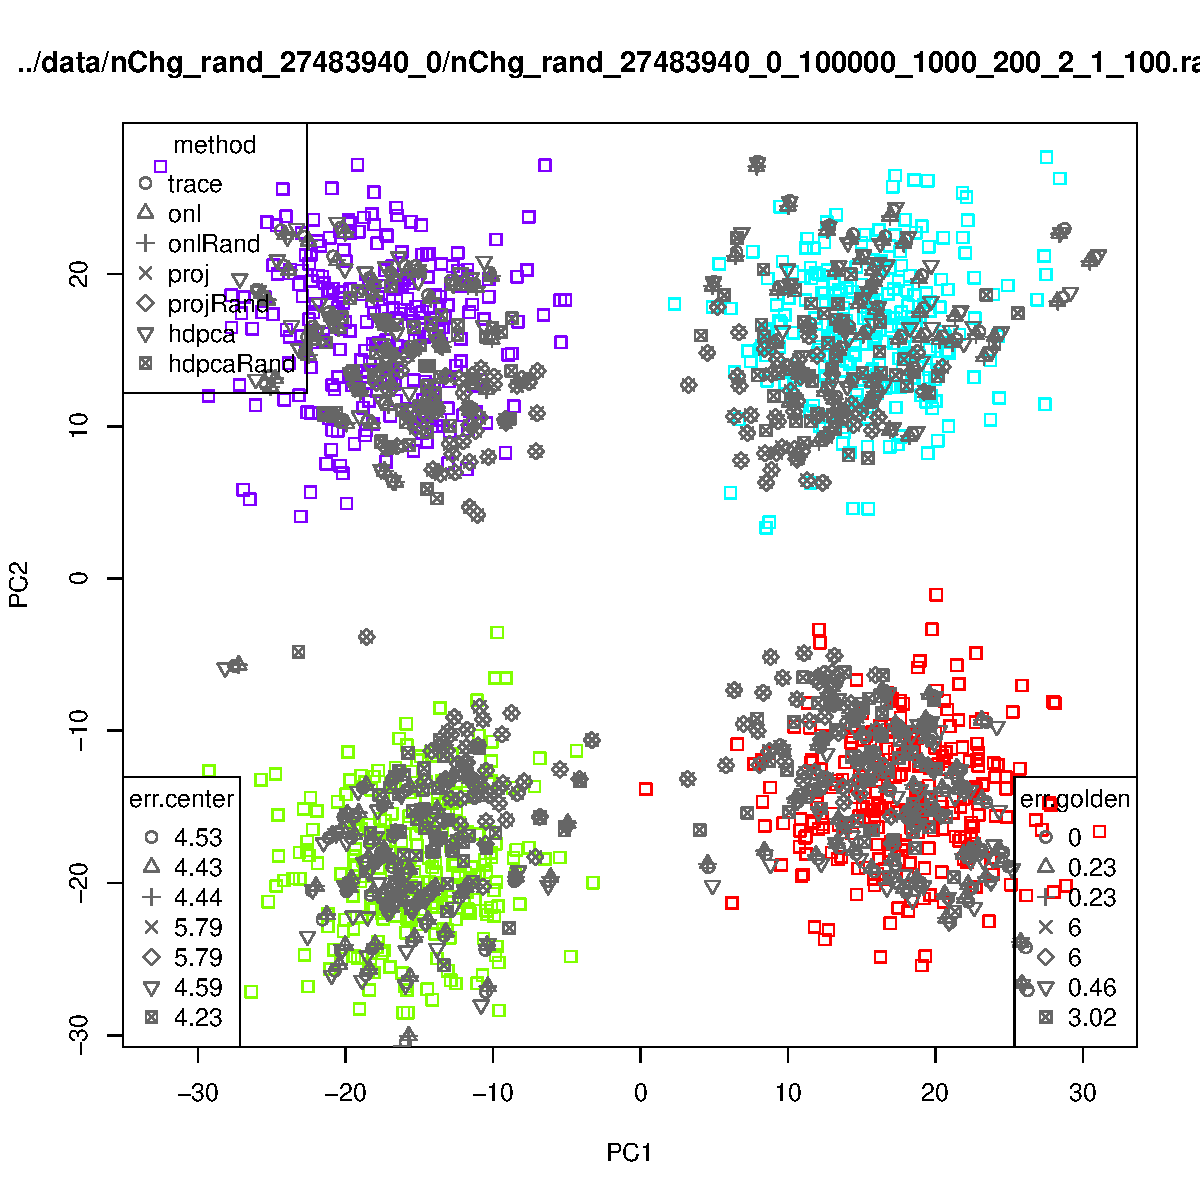
\includegraphics[width=0.98\textwidth]{n1000}
  \caption{
    Predicted PC scores on top of reference PC scores.
    The four populations in the $2 \times 2$ grid simulated by the GGS software can be clearly identified.
    Reference individuals are in color,
    while predicted PC scores for the study individuals are in gray.
    Two measurements of deviations (accuracy) are used.
    The reference center error is the square root of the average squared distance between the study individuals and the population centers, which are the means of the PC scores of the reference individuals by the populations.
    The golden standard error is the square root of the averate squared distance between the study individuals' PC scores predicted by different methods compared to the golden standard result, which in our case is the PC scores predicted by ADP.
    The reference size is 1000 and the study size is 200.
    There are 100,000 loci (1000 per genealogy) and the migration rate is 100.
  }
  \label{fig:n1000}
\end{figure}

\begin{figure}[p]
  \centering
  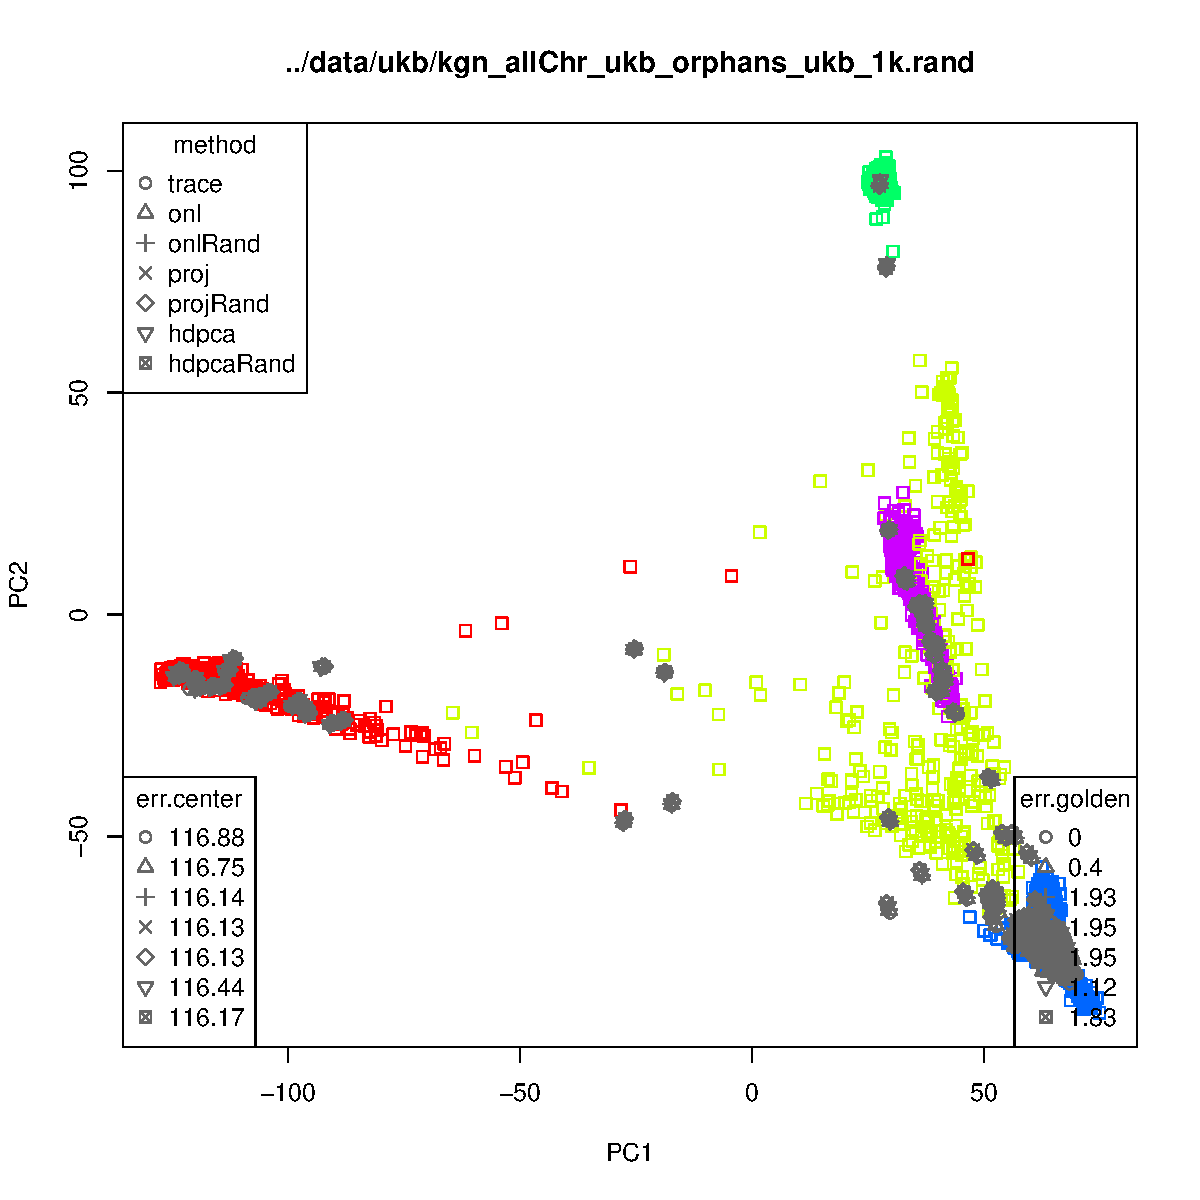
\includegraphics[width=0.98\textwidth]{ukb}
  \caption{
    The reference individuals are from the 1000 Genomes dataset with 2492 unrelated individuals from 5 superpopulations: African, American, East Asian, European, and South Asian. 
    The study sample contain 1000 individuals from the UKBioBank dataset.
    There are about 125,000 loci shared by the reference and study data.
    The golden standard error is the square root of the averate squared distance between the study individuals' PC scores predicted by different methods compared to the golden standard result, which in our case is the PC scores predicted by ADP.
  }
  \label{fig:ukb}
\end{figure}

\begin{figure}[p]
  \centering
  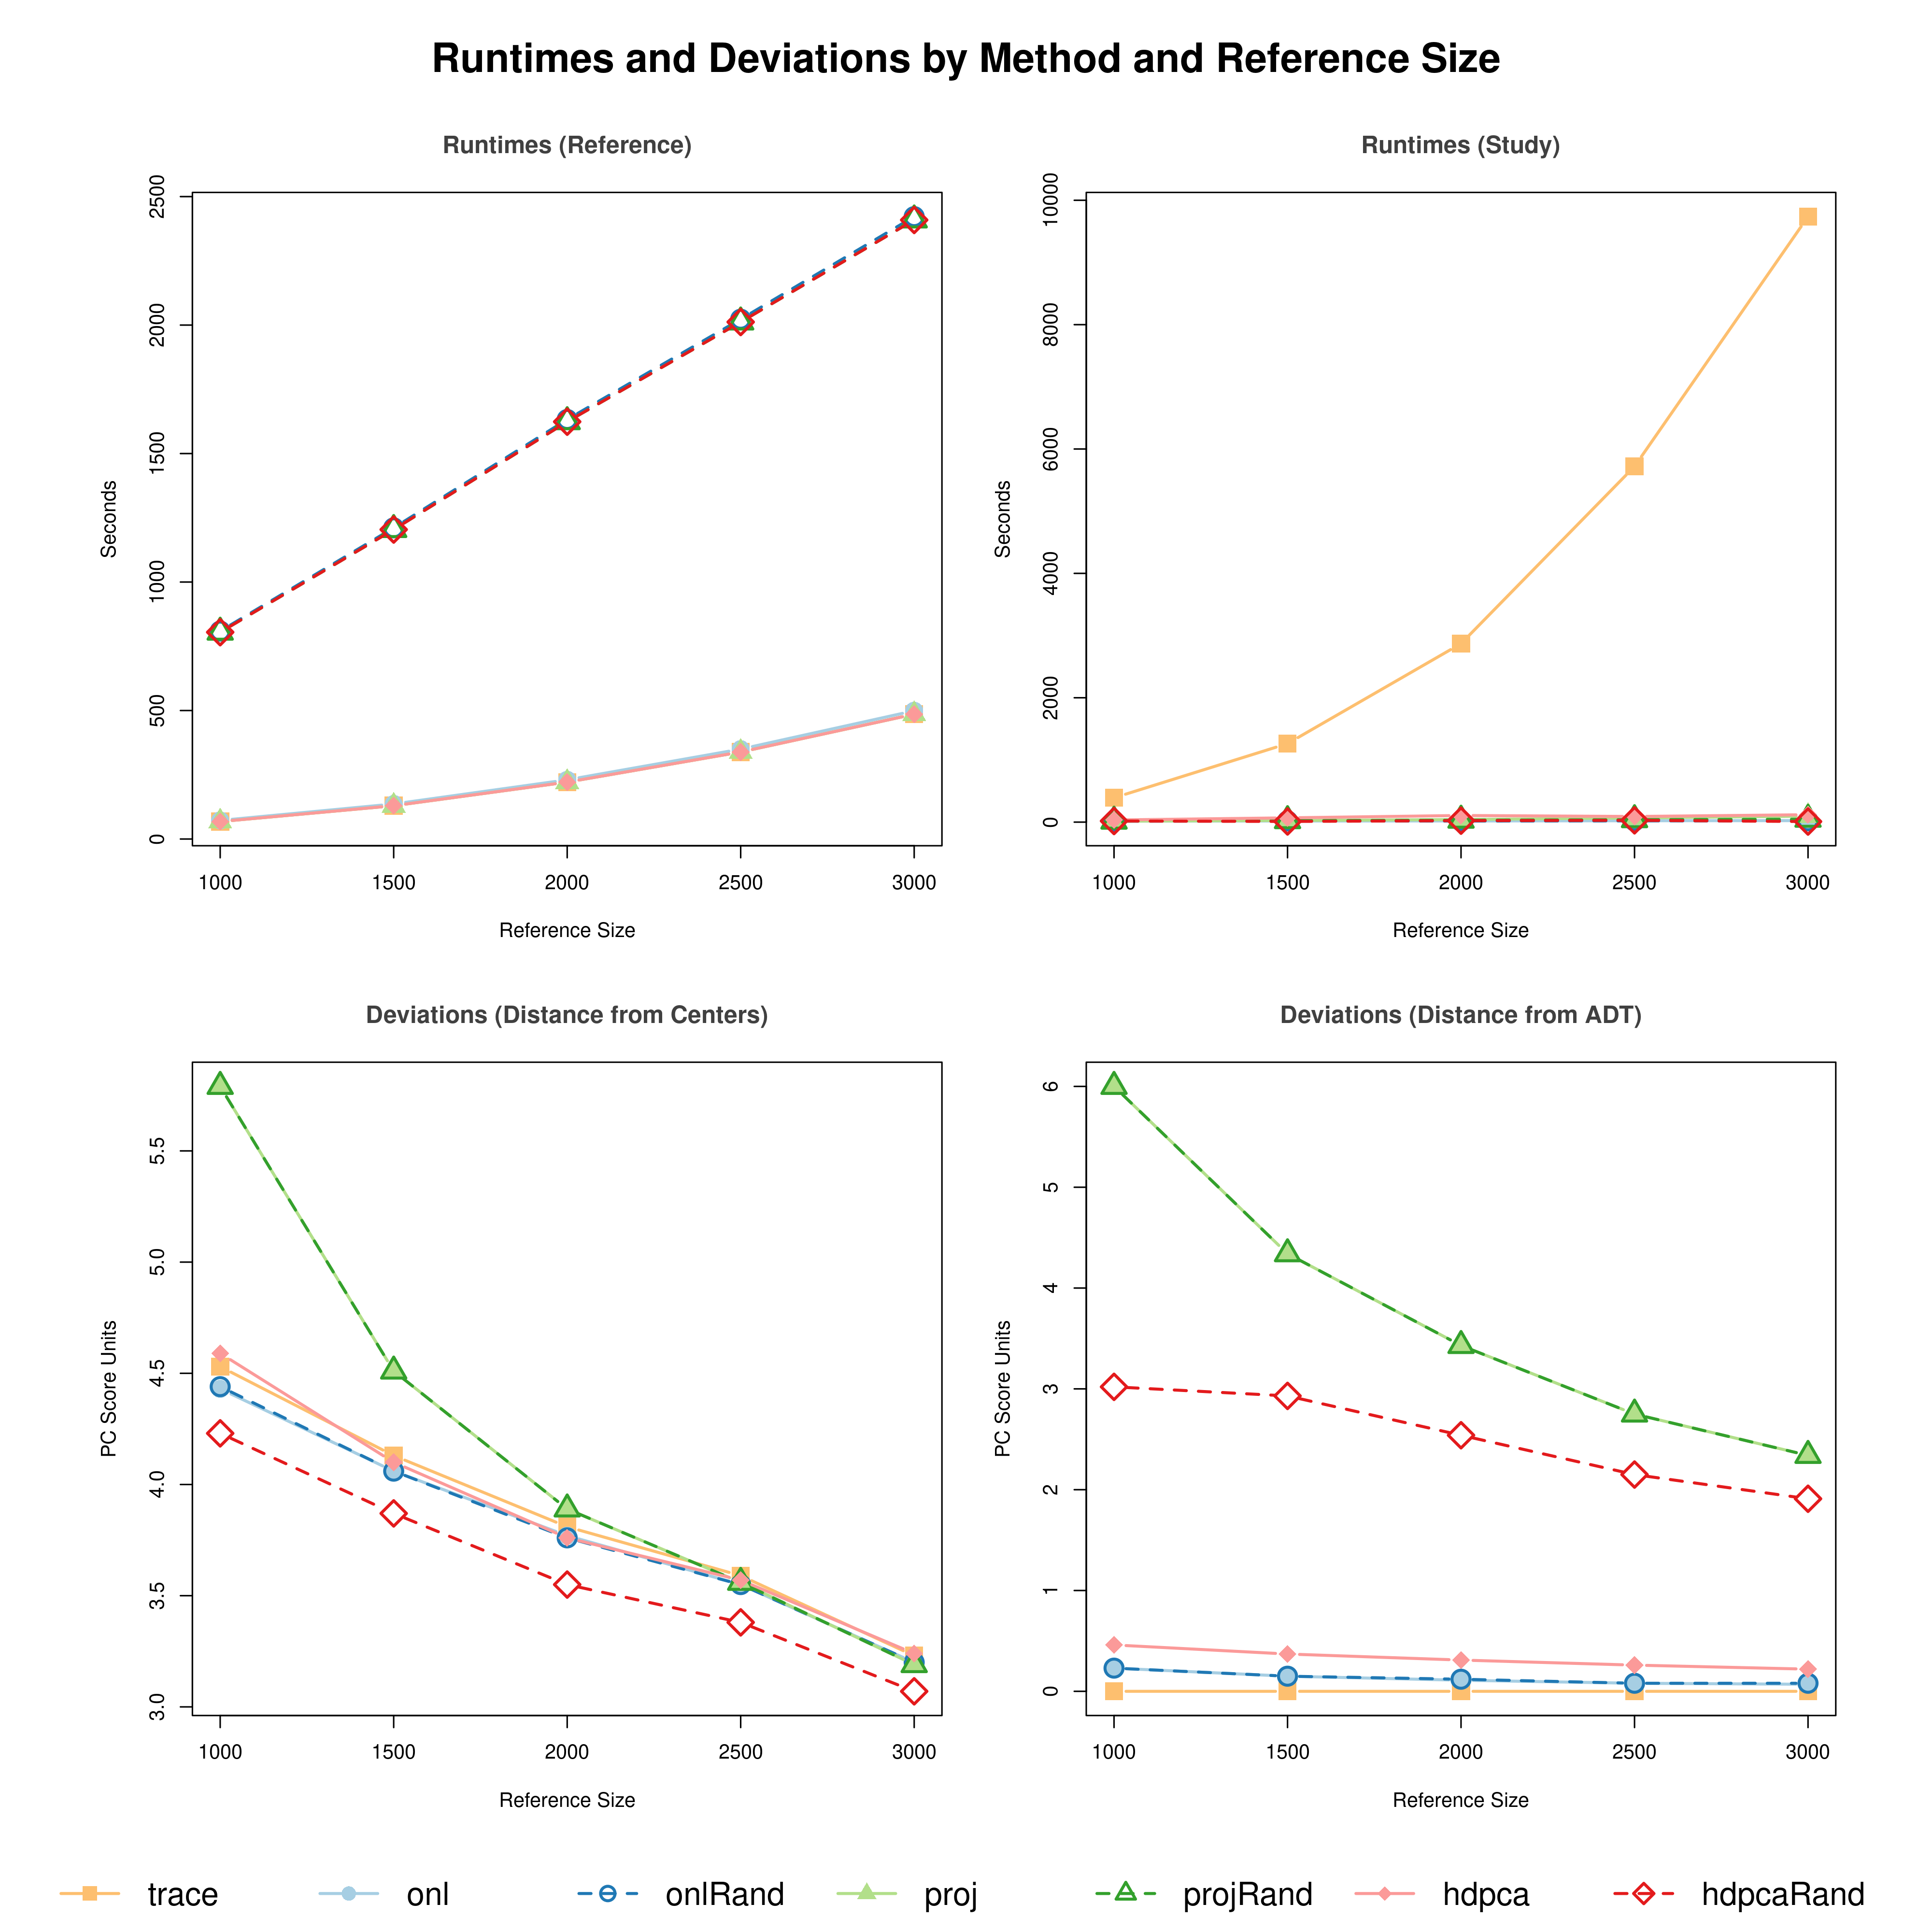
\includegraphics[width=0.98\textwidth]{nChg}
  \caption{
    Runtimes and deviations for different methods as the reference sample size increases.
    The study size is fixed to 200 and the number of SNPs is 100,000 (1000 per genealogy). 
    Simulation is done on a $2 \times 2$ grid with a migration rate of 100 by the GGS software. 
  }
  \label{fig:nChg}
\end{figure}

\begin{figure}[p]
  \centering
  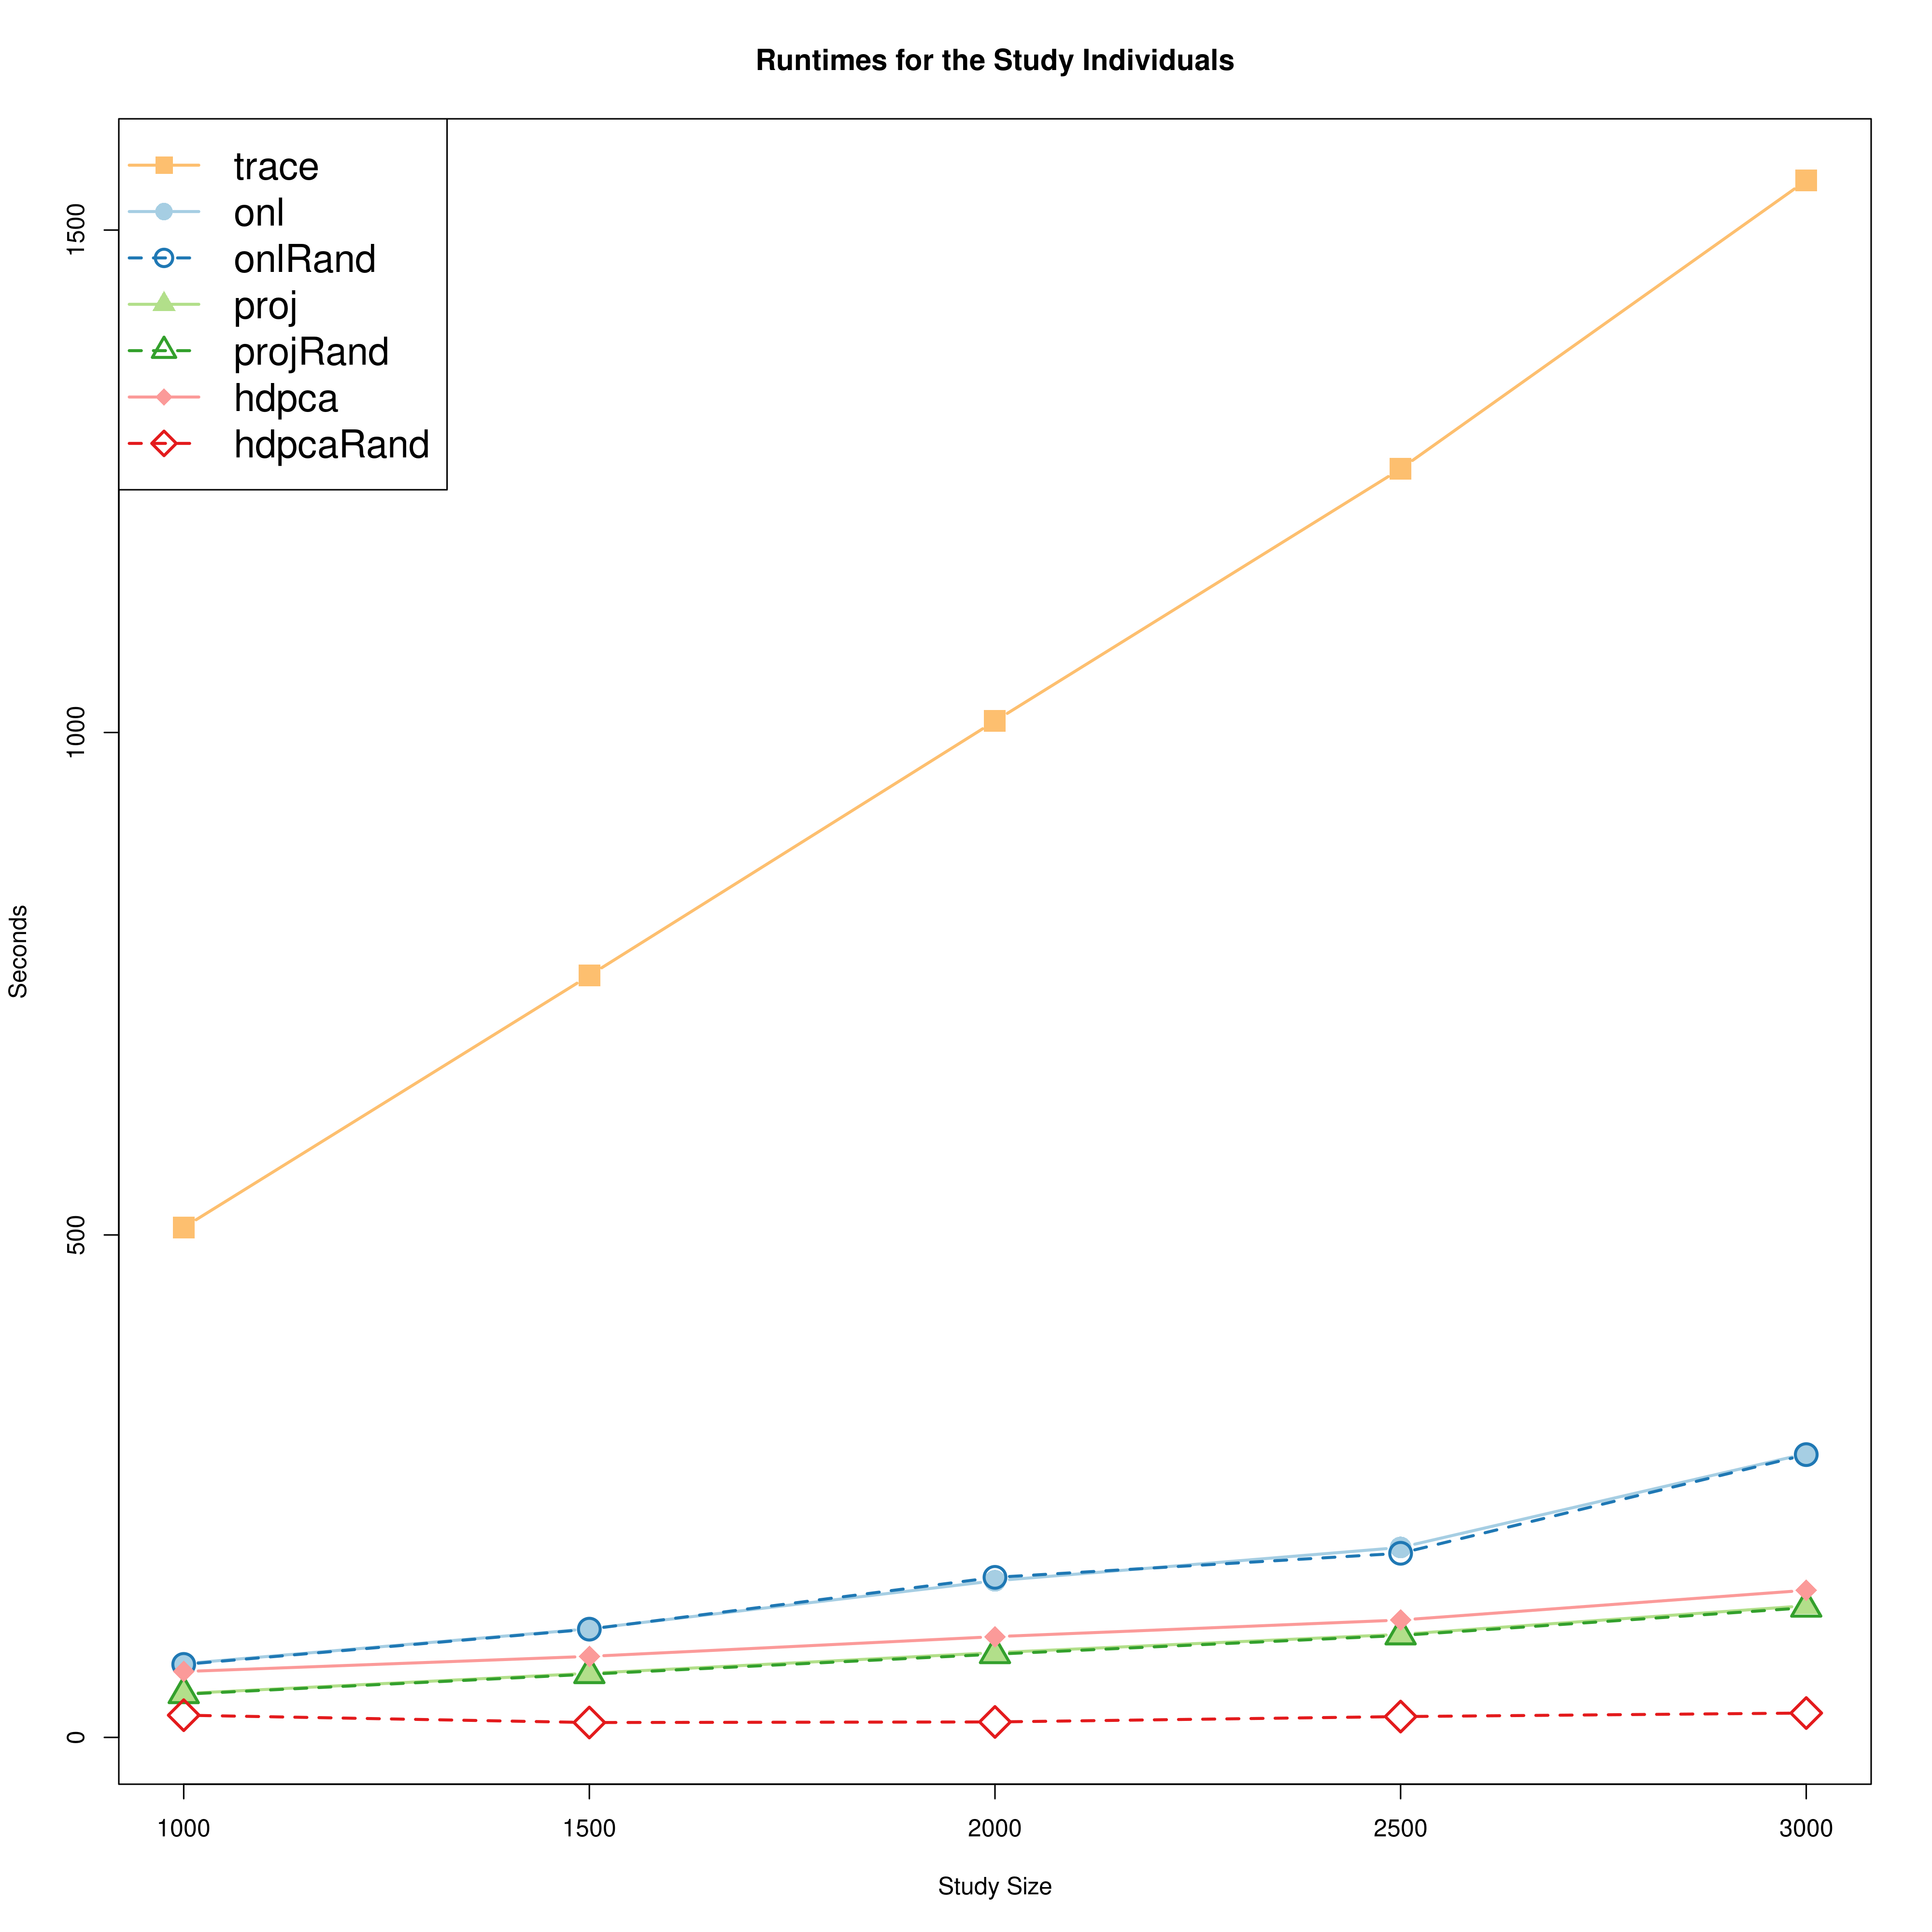
\includegraphics[width=0.98\textwidth]{mChg}
  \caption{
    Runtimes and deviations for different methods as the study sample size increases.
    The reference sample size is fixed to 600 and the number of SNPs is 100,000 (1000 per genealogy).
    Simulation is done on a $2 \times 2$ grid with a migration rate of 100 by the GGS software. 
  }
  \label{fig:mChg}
\end{figure}

% \includegraphics[width=0.98\textwidth]{runtimes_rand}

% \includegraphics[width=0.98\textwidth]{err_refcenter_rand}

% \includegraphics[width=0.98\textwidth]{err_trace_rand}

% \includegraphics[width=0.98\textwidth]{err_refcenter_rand}

% \includegraphics[width=0.98\textwidth]{kgn_allChr_ukb_orphans_ukb_1k_comb}

\newpage
 
% \includegraphics[width=0.98\textwidth]{kgn_allChr_ukb_orphans_ukb_1k_rand}

\newpage


\end{document}
